\documentclass[12pt,twoside]{article}
\usepackage{amsmath, amssymb}
\usepackage[active]{srcltx}
\usepackage{amssymb}
\usepackage{amscd}
\usepackage{makeidx}
\usepackage{amsthm}
\usepackage{algorithm}
\usepackage{algpseudocode}
\usepackage{wrapfig,lipsum}

\usepackage{fancyhdr}
\usepackage{graphics}
%----------------------------------------------------------------------------------------------
\usepackage{amsmath, amssymb}
\usepackage{amsmath}
\usepackage[active]{srcltx}
\usepackage{amssymb}
\usepackage{amscd}
\usepackage{makeidx}
\usepackage[dvips]{graphicx}
\usepackage{latexsym}

\renewcommand{\baselinestretch}{1}
\setcounter{page}{1}
\setlength{\textheight}{21.6cm}
\setlength{\textwidth}{14cm}
\setlength{\oddsidemargin}{1cm}
\setlength{\evensidemargin}{1cm}
\pagestyle{myheadings}
\thispagestyle{empty}
\markboth{\small{Pr\'actica 3. Anthony Steiner.}}{\small{.}}
\date{}
\begin{document}

\begin{figure}[h]
\vspace{-3cm} \hspace{-2cm} \setlength{\unitlength}{1mm}
\begin{picture}(15,25)(-10,0)

\includegraphics[width=16cm,height=3cm]{titulo.jpg}
\end{picture}
\end{figure}

\vspace{0cm}

\centerline{\bf An\'alisis de Algoritmos, Sem: 2022-2, 3CV11, Pr\'actica 3, 30/03/2022}

\centerline{}

%\centerline{}

\begin{center}
\Large{\textsc{Pr\'actica 3: Funciones Recursivas vs Iterativas.}}
\end{center}
\centerline{}
\centerline{\bf {Steiner V\'azquez Anthony Francis}}
\centerline{}
\centerline{$asteinerv1700@alumno.ipn.mx$}


\newtheorem{Theorem}{\quad Theorem}[section]

\newtheorem{Definition}[Theorem]{\quad Definition}

\newtheorem{Corollary}[Theorem]{\quad Corollary}

\newtheorem{Lemma}[Theorem]{\quad Lemma}

\newtheorem{Example}[Theorem]{\quad Example}

\bigskip

\textbf{Resumen:} 
Este documento presenta una comparación de distintos algoritmos que resuelven el problema de dividir 2 números enteros; posteriormente se resolverá el problema de buscar un número en un arreglo de enteros, de manera similar al algoritmo de Búsqueda Binaria, solo que en vez de partir el arreglo en 2, se hará en 3 partes; dicho problema se resolverá de manera recursiva tanto como iterativa, para hacer una comparación de ambos algoritmos.
\newline
\\{\bf Palabras Clave:} C++, Iteratividad, Recursividad, Recurrencias

\section{Introducci\'on}
En la práctica pasada hablamos de lo que era la recursión y la iteración; vimos que los algoritmos pueden expresarse de ambas formas, aunque a veces un problema se puede representar de manera más natural en alguna de las 2 formas, y que a veces varía la complejidad, aunque la complejidad, hasta ahora, solo la hemos podido ver de manera experimental, es decir, a $posteriori$, así que en esta práctica estaremos viendo cómo hacer el análisis a $priori$ de algoritmos recursivos.
\\ Se van a tratar los problemas de la división de 2 números enteros, y también el problema de buscar un número en un arreglo de enteros, vamos a ver diferentes algoritmos para resolver este problema, algunos iterativos, otros recursivos, y haremos una comparación del desempeño que tienen los mismos.
\section{Conceptos B\'asicos}

Vamos a explorar más a fondo la recursividad. Empezando por checar los elementos que componen a una función recursiva.
\newline
\\ Primero tenemos el tamaño del problema. Aunque el tamaño de problema no es propio de los algoritmos recursivos, y ya tratamos esto en una práctica anterior, hay que recordar que el tamaño de problema o tamaño de las entradas de un algoritmo, que como sabemos tiene entrada y salida, y que para resolver un problema debemos entender bien la relación entre las entradas y salidas. Se puede dar como una expresión matemática que involucra cantidades relacionadas a los parametros de entrada y estos determinan la complejidad en término del número de operaciones que el algoritmo debe hacer para resolverlo. Cuando se ocupa la recursión, es especialmente importante puesto que los casos recursivos, y base, claramente, dependen de este. En muchos problemas el tamaño del problema viene en alguno de los parámetros de entrada, pero en otros casos puede estar implícita debido al lenguaje de programación y la forma en que nos permita acceder a través de sintaxis un tamaño en particular.
\newline
\\ Segundo tenemos los casos base. Estos son instancias de problemas que pueden ser resueltos sin uso alguno de recursión, más aún, sin acarrear llamadas recursivas. El tipo más común generalmente está asociado con las instancias más pequeñas del problema, para el cual resulta resolverlo de manera trivial, a veces no se necesita hacer ningún cálculo. Algunas funciones pueden tener más de un caso base, aunque se debe evitar tener casos base incorrectos, o innecesarios, puesto que son redudantes, esto se da cuando estamos poniendo un caso base, que puede ser calculado mediante el caso recursivo; también esto puede restar generalidad, y esto ocasionaría que nuestra función no estuviera definida en todos los puntos, y podría llevar a errores como exceder el máximo número de llamadas a función permitidas. Y peor aún, no tener un caso base, implicaría tener una recursión infinita, y por tanto nunca pararía, lo que resultaría en el mismo error. Habíamos visto que para poder definir una función recursiva es imperativo escribir un caso base, el cual ayuda a terminar de calcular y parar la recursión.
\newline
\\ Tercero tenemos la decomposición del problema. Esto es buscar subproblemas y problemas adicionales; los subproblemas generalmente son similares al problema original pero menores en tamaño. Los subproblemas son ocupados para establecer los casos recursivos. Se puede ver como un proceso que involucra el decrementar el tamaño del problema, y es por eso que es importante determinar correctamente el tamaño del problema. Se suele expresar como una fórmula puesto que es una función matemática.
\newline
\\ Finalmente tenemos los casos recursivos. Definir los casos recursivos, involucra el obtener una forma the construir la solución total del problema original mediante el uso de soluciones de subproblemas similares, que fueron previamente identificados.
\\ Para construir un algoritmo recursivo es importante tener en cuenta sus partes, y observar como modificar, extender, o combinar estas soluciones de los suproblemas para poder resolver el problema original.
\newline
\\ Los algoritmos recursivos pueden ser divididos en categorías, dependiendo de algunos criterios, es decir, existen tipos de algoritmos recursivos, y pueden estar en diferentes categorías.
\\ Primero vamos a ver las recursiones Lineales, estas ocurren cuando las funciones que de alguna manera procesan el resultado de la llamada recursiva, antes de retornar el valor, y solo son llamadas una vez.
\\ Ahora veremos recursión de Cola, este tipo de recursión, es lineal también, así que igualmente solo hace una llamada a sí misma una vez, pero la llamada recursiva es la última operación que se se acarrea del caso recursivo, debido a esto no manipula directamente el resultado de la llamada recursiva. Generalmente estas recursiones modifican el conjunto de argumentos hasta que sea posible calcular la solución de manera simple.
\\ Luego tenemos las recusiones Múltiples, esta ocurre cuando una función se llama a sí misma múltiples veces, para algún caso recursivo.
\\ También se tiene las recursiones mutuas, se dice que un conjunto de funciones son mutuamente recursivas cuando pueden llamarse entre ellas en un orden cíclico. En otras palabras se puede tener una función $f$ que puede llamar a una función $g$, y a su vez puede llamar a una función $h$, y esta termina mandando a llamar a la función $f$. A este tipo de recursión, también se le conoce como recursión indirecta.
\\ Finalmente tenemos la recursión Anidada, esta ocurre cuando un argumento de una función recursiva es definida mediante otra llamada recursiva.
\newline
\\ Los algoritmos recursivos suelen expresarse mediante relaciones de recurrencia, que son funciones matemáticas recursivas, digamos $T$, que describe su costo computacional. Si un algoritmo depende del tamaño de un parámetro de entrada, digamos $n$, entonces $T$ será una función de $n$. Entonces checamos cuántas operaciones hace en los casos base, y se hace una relación; ahora para el caso recursivo simplemente veremos como modifica el tamaño de problema $n$, y se expresa, de nuevo $T$ como una función de $n$ pero con las modificaciones que se le harán durante cada llamada recursiva. Todo junto representa una función por partes, es decir una función definida por múltiples subfunciones, que representan a la función en diferentes intervalos del Dominio de la función.
\newpage
Vamos a ver un ejemplos de relaciones de recurrencia para diferentes algoritmos recursivos de distintas categorías para Fibonacci.
\newline
\\ Fibonacci mediante recursión Lineal:
\begin{equation}
    f(n)=
    \begin{cases}
        1 &\text{si $n$ = 2 o $n$ = 2,} \\
        \lfloor \Phi * f(n-1)+1/2 \rfloor &\text{si $n$ $>$ 2,}
    \end{cases}
\end{equation}
donde $\Phi=\dfrac{1+\sqrt{5}}{2}$, de tal modo que $F(n)=f(n)$.
\newline
\\ Fibonacci mediante recursión de Cola:
\begin{equation}
    f(n,a,b)=
    \begin{cases}
        b &\text{si $n$ = 1,} \\
        f(n-1,a+b,a) &\text{si $n$ $>$ 1.}
    \end{cases}
\end{equation}
así $F(n)=f(n,1,1)$.
\newline
\\ Fibonacci mediante recursión Múltiple:
\begin{equation}
    f(n)=
    \begin{cases}
        1 &\text{si $n$ = 1 o $n$ = 2,} \\
        \text{[$f(\dfrac{n}{2}+1)]^2$} - \text{[$f(\dfrac{n}{2}-1)]^2$}  &\text{si $n$ $>$ 2 y $n$ es par,} \\
        \text{[$f(\dfrac{n+1}{2})]^2$} + \text{[$f(\dfrac{n-1}{2})]^2$}  &\text{si $n$ $>$ 2 y $n$ es impar.}
    \end{cases}
\end{equation}
de este modo $F(n)=f(n)$.
\newline
\\ Fibonacci mediante recursión Mutua:
\begin{equation}
    A(n)=
    \begin{cases}
        0 &\text{si $n$ = 1} \\
        A(n-1)+B(n-1) &\text{si $n$ $>$ 1,}
    \end{cases}
    B(n)=
    \begin{cases}
        1 &\text{si $n$ = 1} \\
        A(n-1) &\text{si $n$ $>$ 1.}
    \end{cases}
\end{equation}
con esto tenemos $F(n)=B(n)+A(n)$.
\newline
\\ Fibonacci mediante recursión Anidada:
\begin{equation}
    f(n,s)=
    \begin{cases}
        1+s &\text{si $n$ = 1 o $n$ = 2,} \\
        f(n-1,s+f(n-2,0)) &\text{si $n$ $>$ 2.}
    \end{cases}
\end{equation}
de modo que $F(n)=f(n,0)$.
\newline
\\ Aunque el hecho de que $T(n)$ describe el costo computacional, aún debemos obtener el la función de su orden de crecimiento. Para hacer esto, se debe resolver la relación de recurrencia, y existen varios métodos para hacer esto.
\\ A la expresión matemática a resolver la vamos a llamar, simplemente, recurrencia, y a la llamada recursiva le vamos a sumar el costo de lo que hace que nuestra llamada recursiva sea ejecutada, y al caso base le llamaremos condición de frontera. Resolver una recurrencia significa encontrar el valor para el $n$-ésimo término generado por la recurrencia.
\newline
\\ Ahora veremos el método de sustitución hacia adeltante.
\\ Para resolver una recurrencia mediante este método se debe empezar por la condición de frontera, e ir calculando los demás términos, de manera sucesiva. Generando así una sucesión, el $n$-ésimo témino de esta sucesión es una función, esta función es la función de complejidad temporal, únicamente, de la llamada recursiva, puesto que la recurrencia puede ser parte de un algoritmo.
\newline
\\ Luego tenemos el método de sustitución hacia atrás.
\\ Este método es el contrario a sustitución hacía delante, aquí se comienza por la recursión original $T(n)$, y se va sustituyendo con el caso recursivo, y así sucesivamente se va sustituyendo hasta que el argumento de la llamada recursiva se convierte en nuestra condición de frontera, de tal manera que podemos observar la función de complejidad temporal hasta ese momento.
\newline
\\ Ahora tenemos el método de Recurrencias Lineales de Orden $N$ con coeficiente constantes homogéneas.
\\ Este método es el análogo a resolver una ecuación diferencial lineal de orden n, con coeficientes constantes homogénea. Aquí tienen la forma: 
\\ $a_n=C_1a_{n-1}+C_2a_{n-2}+\dotsm+C_ka_{n-k}$ donde cada $C_i$ es una constante y $C_k$ es diferente de 0; el valor $k$ es llamado el grado de la relación de recurrencia. Esta expresión tiene un polinomio caracterísitico el cual es: 
\\$r^k=C_1r^{k-1}+C_2r^{k-2}+\dotsm+C_k$, es decir reemplazar $a_i$ con $r^{i-(n-k)}$, ahora debemos calcular las raíces características de la relación de recurrencia, que son las raíces del polinomio caracterísitico.
\\ Para resolver este tipo de recurrencias tenemos los siguientes Teoremas.
\\ \textbf{Teorema 1.} 
\\ Dada una relación de recurrencia $a_n=C_1a_{n-1}+C_2a_{n-2}+\dotsm+C_ka_{n-k}$ con $k$ distintas raíces características $r_1,\dotsc,r_k$.
\\ Entonces la forma cerrada de la solución para $a_n$ tiene la forma: 
\\ $\alpha_1r_1^n+\alpha_2r_2^n+\dotsb+\alpha_kr_k^n$, además dadas $k$ condiciones iniciales, las constantes $\alpha_1,\dotsc,\alpha_k$ están determinadas de manera única.
\\ Si no tenemos $k$ distintas raíces tenemos lo siguiente:
\\ \textbf{Teorema Generalizado.}
\\ Tenemos una relación de recurrencia $a_n=C_1a_{n-1}+C_2a_{n-2}+\dotsm+C_ka_{n-k}$ con $t$ raíces características distintas $r_1,\dotsc,r_k$, con multiplicidades $m_1,\dotsc,m_k$. Entonces la solución tiene la forma:
\[ a_n = \sum_{i=0}^{t} (\alpha_{i,0}+\alpha_{i,1}\cdot n+\dotsb+\alpha_{i,m_{i-1}}\cdot n^{m_i-1})r_i^n  \]
Finalmente con la condiciones iniciales, armamos un sistema de ecuaciones, y al resolverlo, tendremos los valores para cada $C_i$. Con lo cual tendríamos nuestra función de complejidad.
\newline
\\ Ahora tenemos el método de Recurrencias Lineales de Orden $N$ con coeficiente constantes no homogéneas.
\\ Si tenemos una relación de recurrencia lineal de coeficientes constantes como: $a_n=C_1a_{n-1}+C_2a_{n-2}+\dotsm+C_ka_{n-k}+F(n)$, se dice que es no homogénea. La relación de recurrencia que se obtiene al eliminar $F(n)$ se conoce como la relación de recurrencia homogénea asociada. Para resolver recurrencias de este tipo, también recurriremos al análogo en ecuaciones diferenciales del mismo tipo, donde combinaremos la solución de la homogénea, con una solución particular. Para ello usaremos los siguientes teoremas:
\\ \textbf{Teorema 1.}
\\ Se supone que $a_n=C_1a_{n-1}+C_2a_{n-2}+\dotsm+C_ka_{n-k}+F(n)$ tiene una solución particular $a_n^p$, y $a_n^h$ es la solución de la recurrencia homogénea asociada. Entonces toda solución tiene la forma: $a_n^p+a_n^h$. Si podemos encontrar una solución particular, entonces, mecánicamente podemos encontrar una solución que satisaface las condiciones iniciales. Se encuentra de la siguiente manera.
\\ \textbf{Teorema 2.}
\\ Considere $a_n=C_1a_{n-1}+C_2a_{n-2}+\dotsm+C_ka_{n-k}+F(n)$ donde: 
\\ $F(n)=(b_tn^t+b_{t-1}n^{t-1}+\dotsb+b_1n+b_0)s^n$
\\ Caso 1. Si $s$ no es una raíz de la ecuación característica asociada, entonces existe una solución particular de la forma:
\\ $(p_tn^t+p_{t-1}n^{t-1}+\dotsb+p_1n+p_0)s^n$
\\ Caso 2. Si $s$ es una raíz con multiplicidad $m$ de la ecuación caracterísitica, entonces existe una solución de la forma:
\\ $n^m(p_tn^t+p_{t-1}n^{t-1}+\dotsb+p_1n+p_0)s^n$
\\ Ahora solo igualamos la forma de la solución particular con nuestra recurrencia, y resolvemos para los $p_i$ acomodando todo para que este igualado a 0. Y esa sería la función de complejidad temporal.
\newline
\\ Ahora se presenta el método de árboles de recurrencia.
\\ Este método ocupa el construir un árbol de sustituir los valores de una recurrencia con la forma $T(n)=aT(n/b)+f(n)$, de tal manera que cada nodo del árbol tendrá $a$ hijos, y los valores de esos nodos serán las $f(n)$ evaluadas en la $T$ de ese nivel. Luego se busca obtener cuál es el nivel del árbol donde solo hay $T(1)$, luego vemos cuántas operaciones realiza por cada nivel, se suman, y así se obtiene la función de complejidad.
\newline
\\ Ahora veremos el método heúristico.
\\ Para ocupar este método se propone una función $f(n)$, la cuál checaremos por medio de inducción matemática si es la complejidad de nuestro algoritmo, en caso contrario, se prueba con otra función y así sucesivamente, de tal modo que se checa a prueba y error.
\newline
\\ Finalmente tenemos el método Maestro.
\\ Para este método haremos uso del Teorema Maestro, que es el siguiente:
\\ \textbf{Teorema Maestro.}
\\ Sean $a \leq 1$ y $b>1$ constantes. Sea $f(n)$ una función, y sea $T(n)$ una función definida sobre los números enteros no negativos, por la relación de recurrencia:
\begin{equation}
    T(n)=
    \begin{cases}
        d &\text{$d>0$} \\
        aT(\frac{n}{b})+f(n) &\text{o.c,}
    \end{cases}
\end{equation}
donde $\frac{n}{b}$ puede ser $\lfloor \frac{n}{b} \rfloor$ o $\lceil \frac{n}{b} \rceil$. Entonces $T(n)$ está acotado asintóticamente por:
\\ Caso 1. Si $f(n)= O(n^{\log_ba-\epsilon})$ para algún $\epsilon>0$, entonces $T(n)=\Theta(n^{\log_ba})$.
\\ Caso 2. Si $f(n)= \Theta(n^{\log_ba})$, entonces $T(n)=\Theta(n^{\log_ba}\cdot \log n)$.
\\ Caso 3. Si $f(n)= \Omega(n^{\log_ba+\epsilon})$ para algún $\epsilon>0$, y si $a\cdot f(\frac{n}{b})\leq c\cdot f(n)$ para alguna constante $c<1$, y todas la $n$ suficientemente grandes, entonces $T(n)=\Theta(f(n))$.
\newline
\\ Ahora vamos a ver los tipos de recurrencias comunes.
\\ Primero vamos a ver Decremento por 1.
\\ La cual es una recurrencia de la forma $T(n)=T(n-1)+f(n)$, este tipo de recurrencia se puede resolver por el método de sustitución hacia atrás, lo que nos da como resultado, que para saber la complejidad de este tipo de recurrencia basta con saber el valor de: $\sum_{j=1}^{n} f(j)$.
\newline
\\ Luego tenemos Decremento por un factor constante.
\\ Estas son recurrencias de la forma $T(n)=T(\frac{n}{b})+f(n)$, con $b>1$, igualmente mediante sustitución hacia atrás, haciendo el cambio de variable $n=b^k$, i.e. $k=\log_bn$, tenemos que la función de complejidad es:  $\sum_{j=1}^{k} f(b^j)$ o lo que es lo mismo:  $\sum_{j=1}^{\log_bn} f(b^j)$.
\newline
\\ Finalmente tenemos las recurrencias de Divide y Vencerás.
\\ Una recurrencia Divide y Vencerás es de la forma: $T(n)=aT(\frac{n}{b})+f(n)$ con $a\geq 1$ y $b\geq 2$. Igualmente mediante sustitución hacia atrás, con el cambio de variable $n=b^k$, tenemos que la función de complejidad es: $n^{\log_ba}\sum_{j=1}^{log_bn} \frac{f(b^j)}{a^j}$.
\newpage
Con esto vamos a ver los siguientes algoritmos y vamos a calcular su orden de complejidad de cada uno.
\\ Empezaremos con el problema de la división de 2 números enteros, del cual veremos 3 algoritmos.
\newline
\\ Tenemos el algoritmo 1, que llamaremos División 1, que es iterativo.
\begin{algorithm}
    \caption{Division1($n,div,res$):}
    \begin{algorithmic}
        \State $q \gets 0$
        \While{$n\geq div$}
            \State $n \gets n-div$
            \State $q \gets q+1$
        \EndWhile
        \State $res \gets n$
        \State \textbf{return} $q$
    \end{algorithmic}
\end{algorithm}
\\ Veamos su funcionamiento, si $n$=3, y $div$ = 1, entonces el algoritmo comienza poniendo la variable auxiliar $q$ en 0, después itera mientras que $n$ sea menor o igual a $div$, haciendo que $n$ ahora valga $n-div$ es decir para la primera iteración $n$ valdrá 2, y le aumenta 1 a $q$ es decir ahora valdrá 1, luego para la 2nda iteración $n$ sigue siendo mayor o igual a $div$ por lo tanto entra al ciclo y ahora $n$ valdrá 1, y $q$ 2, finalmente entra por última vez al ciclo, puesto que $n$ ahora es igual a $div$, por lo tanto $n$ ahora vale 0, y $q$ vale 3, por lo tanto nuestra variable $res$ que tendrá el residuo de la operación será igual a $n$, y retoranmos $q$, lo que nos diría que el resultado de dividir 3 entre 1, es 3, con residuo 0, por lo tanto el algoritmo es correcto.
\newpage
Ahora veremos el algiritmo 2, que llamaremos División 2, también iterativo.
\begin{algorithm}
    \caption{Division2($n,div,r$):}
    \begin{algorithmic}
        \State $dd \gets div$
        \State $q \gets 0$
        \State $r \gets n$
        \While{$dd\leq n$}
            \State $dd \gets 2\cdot dd$
        \EndWhile
        \While{$dd> div$}
            \State $dd \gets \frac{dd}{2}$
            \State $q \gets 2\cdot q$
            \If{$dd\leq r$}
                \State $r \gets r-dd$
                \State $q \gets q+1$
            \EndIf
        \EndWhile
        \State \textbf{return} $q$
    \end{algorithmic}
\end{algorithm}
\\ Este algoritmo comienza declarando una variable auxiliar $dd$ e inicilizandola con el valor de $div$, la variable auxiliar $q$ con 0, y $r$ con $n$, la cual será nuestro residuo. Después iteramos mientras que $dd$ sea menor o igual a $n$ duplicando su valor cada vez. Posteriormente, iteramos mientras que $dd$ sea mayor que $div$, reduciendo a la mitad el valor de $dd$ en cada iteración, luego duplicando el valor de $q$, y luego checamos si $dd$ es menor o igual a $r$ en tal caso restamos $dd$ de $r$, y le aumentamos 1 a $q$, finalmente retornamos $q$. Veamos en funcionamiento este algoritmo para cuando $n=3$ y $div=1$, tenemos que $dd$ será 1, $q$ será 0, y $r$ será 3. Así en el primer ciclo, para la primer iteración $dd$ valdrá 2, vuelve a entrar y aumenta a 4, y se sale del ciclo. Luego para el siguiente ciclo, como $dd$ vale 4 es mayor que $div$ que vale 1, entonce entra, y reduce el valor de $dd$ a 2, luego duplica el valor de $q$ pero sigue en 0, luego checamos si $dd$ es menor o igual a $r$ que vale 3, lo cuál es cierto, entonces ahora $r$ vale 1, y aumentamos 1 a $q$ por lo tanto ahora vale 1, en la segunda iteración $dd$ que vale 2, sigue siendo mayor a $div$ que vale 1, entonces entra y ahora $dd$ vale 1, y $q$ ahora vale 2, checamos si $dd$ que vale 1 es menor o igual que $r$ que vale 1, lo cual es cierto entonces entra, y ahora $r$ vale 0, y $q$ vale 3. Ya no se cumple y deja de iterar, por lo que solo restar retornar $q$ es decir 3. Lo cual nos dice que el resultado de dividir 3 entre 1, es 3 con residuo de 0, lo cual indica que el algoritmo es correcto.
\newpage
Finalmente veremos el algoritmo 3, que llamaremos División 3, recursivo.
\begin{algorithm}
    \caption{Division3($n,div$):}
    \begin{algorithmic}
        \If{$div>n$}
            \State \textbf{return} $0$
        \Else
            \State \textbf{return} $1+Division3(n-div,div)$
        \EndIf
    \end{algorithmic}
\end{algorithm}
\\ Este algoritmo recursivo simplemente checa si $div$ es mayor a $n$ en tal caso simplemente retorna 0, pero en caso contrario retorna 1 + la llamada recursiva con tamaño n-div. Veamos cómo funciona si $n$ es igual a 3, y $div$ vale 1. Primero checamos si $div$ es mayor a $n$ lo cual no se cumple, por lo tanto entra al else, y retorna 1 + Division3(2,1), la cual, también, hay que calcular, así que ahora checaremos Division3(2,1), aquí $n$ es igual a 2, y $div$ sigue valiendo 1, tampoco se cumple que $div$ sea mayor que $n$, entonces retornamos $1+Division3(1,1)$ ahora debemos calcular Division3(1,1), como tampoco se cumple que $div$ sea mayor que $n$, retorna $1+Division3(0,1)$, para este caso $div$ es mayor a $n$, por lo tanto retorna 0, ahora se puede calcular todo, que sería sumar $1+1+1+0$, lo cual es 3, que es el resultado de dividir 3 entre 1, por lo tanto el algoritmo es correcto. 
\newpage
Ahora veremos el 2ndo problema, es decir el de buscar un número en un arreglo de enteros.
\\ En su forma Recursiva:
\begin{algorithm}
    \caption{BusquedaEn3Bloques($A,busca,inicio,final$):}
    \begin{algorithmic}
        \If{$inicio > final$} 
            \State \textbf{return} $-1$
        \Else
            \State $i \gets (final-inicio)/3+inicio$
            \State $j \gets 2*(final-inicio)/3+inicio$
            \If{$busca == A[i]$}
                \State \textbf{return} $i$
            \ElsIf{$busca == A[j]$}
                \State \textbf{return} $j$
            \ElsIf{$busca > A[j]$}
                \State $inicio \gets j + 1$
                \State \textbf{return} $BusquedaEn3BloquesRecursiva(A, busca, inicio, final)$
            \ElsIf{$busca > A[i]$}
                \State $inicio \gets i + 1$
                \State $final \gets j - 1$
                \State \textbf{return} $BusquedaEn3BloquesRecursiva(A, busca, inicio, final)$
            \Else
                \State $final \gets i - 1$
                \State \textbf{return} $BusquedaEn3BloquesRecursiva(A, busca, inicio, final)$
            \EndIf
        \EndIf 
    \end{algorithmic}
\end{algorithm}
\\ Este algoritmo parte en 3 bloques nuestro arreglo, y checa si está en la 1ra parte, o en la 2nda parte, si no está ahí, entonces checa el rango en el que se encuntra nuestro valor, y checa ahora solo en ese pedazo volviendo a partirlo en 3, y así, hasta que o encuntra el valor buscado, o no lo encuntra cuando los indices se cruzan.
\\ Por ejemplo si tenemos un arreglo con los elementos: 1,2,3,4,5,6,7,8,9,10; nuestras variables $i,j$ toman los valores de 4, y 8 respectivamente, supongamos que buscamos el 6, entonces ahora solo checara entre el subarreglo 5,6,7, en este caso $i$ valdría 5, y $j$ valdría 7, finalmente solo checa en el subarreglo 6; como este es el valor que estabamos buscando entonces regresa su índice.
\newpage
En su forma Iterativa:
\begin{algorithm}
    \caption{BusquedaEn3Bloques($A,n,busca$):}
    \begin{algorithmic}
        \State $inicio \gets 0$
        \State $final \gets n-1$
        \While{$inicio \leq final$}
            \State $i \gets (final-inicio)/3+inicio$
            \State $j \gets 2*(final-inicio)/3+inicio$
            \If{$busca == A[i]$}
                \State \textbf{return} $i$
            \ElsIf{$busca == A[j]$}
                \State \textbf{return} $j$
            \ElsIf{$busca > A[j]$}
                \State $inicio \gets j + 1$
            \ElsIf{$busca > A[i]$}
                \State $inicio \gets i + 1$
                \State $final \gets j - 1$
            \Else
                \State $final \gets i - 1$
            \EndIf
        \EndWhile
        \State \textbf{return} $-1$
    \end{algorithmic}
\end{algorithm}
\\ El algoritmo funciona exactamente igual que en su forma recursiva, simplemente está escrito de manera iterativa.
\newline
\\ Finalmente vamos a calcular sus ordenes de complejidad.

\section{Experimentaci\'on y Resultados}
Vamos a empezar con nuestro 1er problema, la división de 2 números enteros, y los 3 algoritmos que ya presentamos, para todos los algoritmos, el tamaño del problema es $n$, el mejor caso es cuando $div$ es mayor a $n$, y el peor caso cuando $div$ vale 1.
\newline
\\ Para División1:
\\ Veamos en ejecución este algoritmo.
\newpage
\begin{figure}[h]
    \vspace{3cm} \hspace{-2cm} \setlength{\unitlength}{1mm}
        \begin{picture}(15,25)(-35,0)
            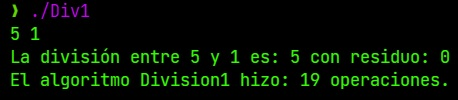
\includegraphics[width=10cm,height=5cm]{D1_Ex.jpg}
        \end{picture}
    \end{figure}
    \vspace{-0.7cm}
    \begin{center}
        Figura 1. Ejecución de Division1
    \end{center}
    \medskip
Ahora veamos su complejidad temporal a $priori$.
\begin{figure}[h]
    \vspace{3cm} \hspace{-2cm} \setlength{\unitlength}{1mm}
        \begin{picture}(15,25)(-35,0)
            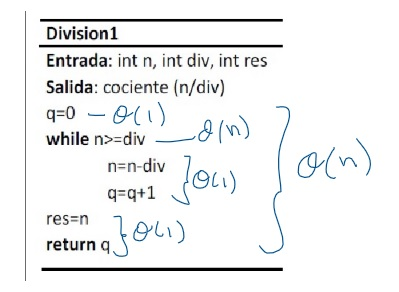
\includegraphics[width=10cm,height=5cm]{D1_PR.jpg}
        \end{picture}
    \end{figure}
    \vspace{-0.7cm}
    \begin{center}
        Figura 2. Análisis a $priori$ de Division1
    \end{center}
    \medskip
Ahora realizaremos el análisis a $posteriori$
\\ Para el mejor caso:
\newpage
\begin{table}[htbp]
    \begin{center}
        \begin{tabular}{|c|c|}
            \hline
            \textbf{div} & \textbf{\# operaciones} \\
            \hline \hline
            0 &	4 \\ \hline
            10 & 4 \\ \hline
            20 &	4 \\ \hline
            30 &	4 \\ \hline
            40 &	4 \\ \hline
            50 &	4 \\ \hline
            60 & 4 \\ \hline
            70 & 4 \\ \hline
            80 & 4 \\ \hline
            90 & 4 \\ \hline
            100 & 4 \\ \hline
        \end{tabular}
        \caption{Mediciones para el mejor caso de Division1}
        \label{tabla:analisisDiv1BC}
    \end{center}
\end{table}
Así proponemos la función $f(n)=4$.
\begin{figure}[h]
    \vspace{3cm} \hspace{-2cm} \setlength{\unitlength}{1mm}
        \begin{picture}(15,25)(-35,0)
            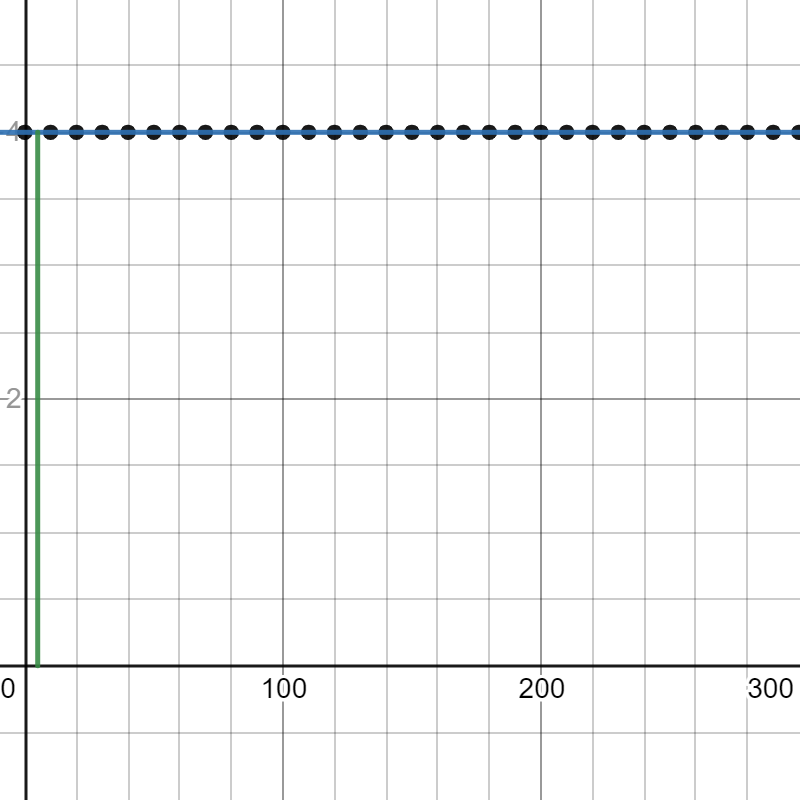
\includegraphics[width=10cm,height=5cm]{D1_P_BC.png}
        \end{picture}
    \end{figure}
    \vspace{-0.7cm}
    \begin{center}
        Figura 3. Gráfica de la función $f(n)=4$.
    \end{center}
    \medskip
Vemos que la función pasa por todos los puntos. De la definición de $\Omega$:
\\ Necesitamos encontrar un $c_1g(n) \le 4$  $\forall n \geq n_1$, de ah\'i que:
\\ $3(1) \le 4 $ $\forall n \geq 1$, entonces $c_1 = 3$, $g(n)=1$, y $n_1=1$ $\therefore$ $f(n)=4 \in \Omega(1)$.
\newpage
Para el peor caso:
\begin{table}[htbp]
    \begin{center}
        \begin{tabular}{|c|c|}
            \hline
            \textbf{div} & \textbf{\# operaciones} \\
            \hline \hline
            0 &	4 \\ \hline
            10 & 19 \\ \hline
            20 &	34 \\ \hline
            30 &	49 \\ \hline
            40 &	64 \\ \hline
            50 &	79 \\ \hline
            60 & 94 \\ \hline
            70 & 109 \\ \hline
            80 & 124 \\ \hline
            90 & 139 \\ \hline
            100 & 154 \\ \hline
        \end{tabular}
        \caption{Mediciones para el peor caso de Division1}
        \label{tabla:analisisDiv1WC}
    \end{center}
\end{table}
\\Así proponemos la función $f(n)= 2n$.
\begin{figure}[h]
    \vspace{3cm} \hspace{-2cm} \setlength{\unitlength}{1mm}
        \begin{picture}(15,25)(-35,0)
            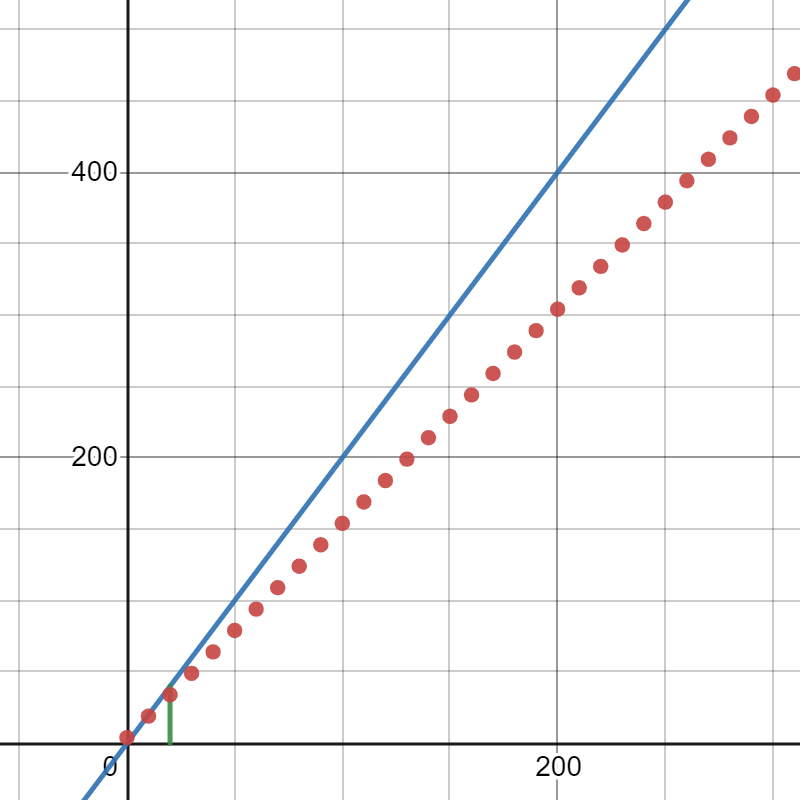
\includegraphics[width=10cm,height=5cm]{D1_P_WC.png}
        \end{picture}
    \end{figure}
    \vspace{-0.7cm}
    \begin{center}
        Figura 4. Gráfica de la función $f(n)=2n$.
    \end{center}
    \medskip
Podemos observar que algunos de estos puntos pasan por la función, y los demás están por debajo. De la definición de $O$:
\\ Necesitamos encontrar un $c_1g(n) \geq 2n$  $\forall n \geq n_1$, de ah\'i que:
\\ $2n \le 3n $ $\forall n \geq 20$, entonces $c_1 = 3$, $g(n)=n$, y $n_1=20$ $\therefore$ $f(n)=2n \in O(n)$.
\newpage
Para División2:
\\ Veamos en ejecución este algoritmo.
\begin{figure}[h]
    \vspace{3cm} \hspace{-2cm} \setlength{\unitlength}{1mm}
        \begin{picture}(15,25)(-35,0)
            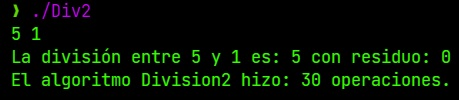
\includegraphics[width=10cm,height=5cm]{D2_Ex.jpg}
        \end{picture}
    \end{figure}
    \vspace{-0.7cm}
    \begin{center}
        Figura 5. Ejecución de Division2
    \end{center}
    \medskip
Ahora veamos su complejidad temporal a $priori$.
\begin{figure}[h]
    \vspace{3cm} \hspace{-2cm} \setlength{\unitlength}{1mm}
        \begin{picture}(15,25)(-35,0)
            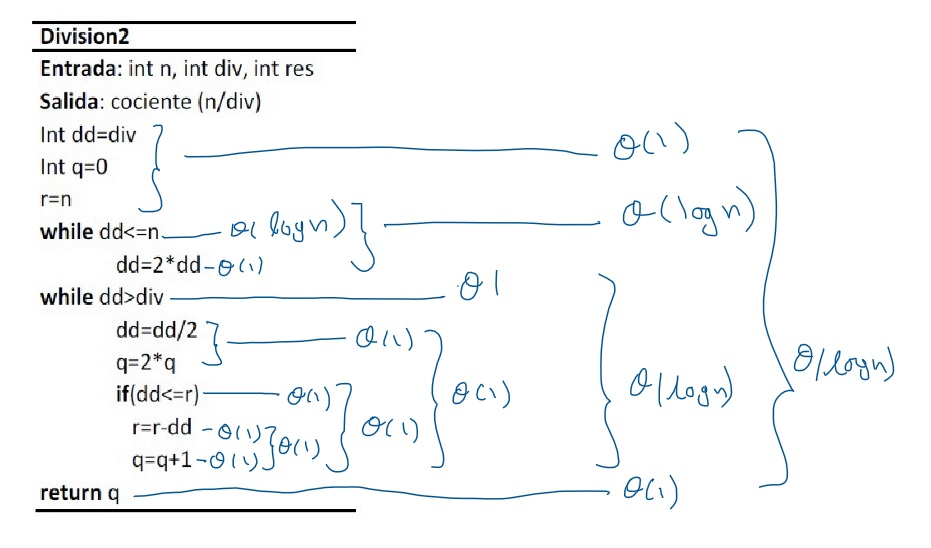
\includegraphics[width=10cm,height=5cm]{D2_PR.jpg}
        \end{picture}
    \end{figure}
    \vspace{-0.7cm}
    \begin{center}
        Figura 6. Análisis a $priori$ de Division2
    \end{center}
    \medskip
Ahora realizaremos el análisis a $posteriori$
\\ Para el mejor caso:
\newpage
\begin{table}[htbp]
    \begin{center}
        \begin{tabular}{|c|c|}
            \hline
            \textbf{div} & \textbf{\# operaciones} \\
            \hline \hline
            0 &	6 \\ \hline
            10 & 6 \\ \hline
            20 &	6 \\ \hline
            30 &	6 \\ \hline
            40 &	6 \\ \hline
            50 &	6 \\ \hline
            60 & 6 \\ \hline
            70 & 6 \\ \hline
            80 & 6 \\ \hline
            90 & 6 \\ \hline
            100 & 6 \\ \hline
        \end{tabular}
        \caption{Mediciones para el mejor caso de Division2}
        \label{tabla:analisisDiv2BC}
    \end{center}
\end{table}
Así proponemos la función $f(n)=6$.
\begin{figure}[h]
    \vspace{3cm} \hspace{-2cm} \setlength{\unitlength}{1mm}
        \begin{picture}(15,25)(-35,0)
            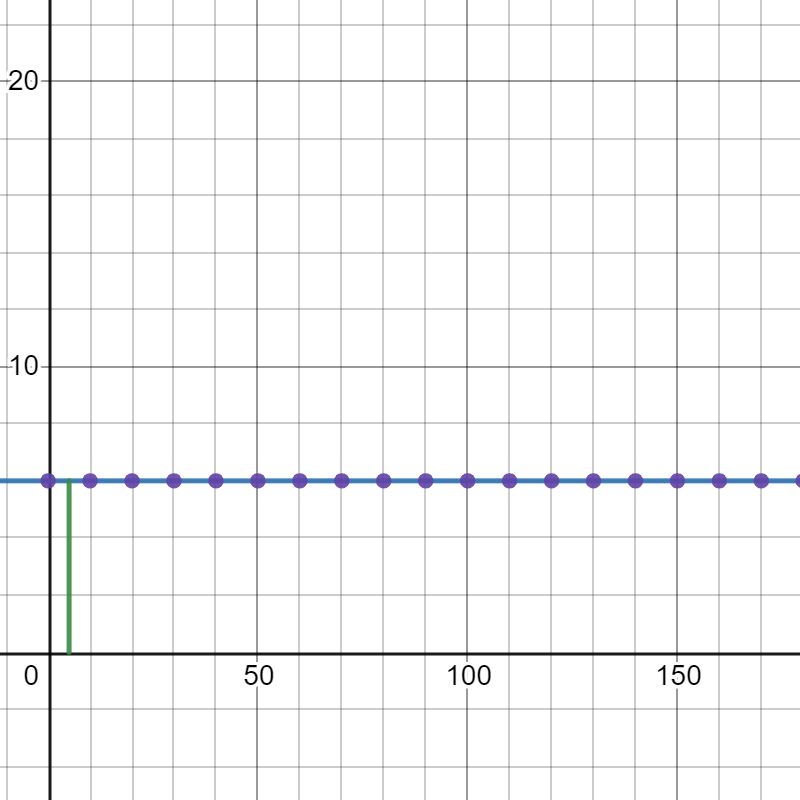
\includegraphics[width=10cm,height=5cm]{D2_P_BC.png}
        \end{picture}
    \end{figure}
    \vspace{-0.7cm}
    \begin{center}
        Figura 7. Gráfica de la función $f(n)=6$.
    \end{center}
    \medskip
Vemos que la función pasa por todos los puntos. De la definición de $\Omega$:
\\ Necesitamos encontrar un $c_1g(n) \le 6$  $\forall n \geq n_1$, de ah\'i que:
\\ $5(1) \le 6 $ $\forall n \geq 1$, entonces $c_1 = 5$, $g(n)=1$, y $n_1=1$ $\therefore$ $f(n)=6 \in \Omega(1)$.
\newpage
Para el peor caso:
\begin{table}[htbp]
    \begin{center}
        \begin{tabular}{|c|c|}
            \hline
            \textbf{div} & \textbf{\# operaciones} \\
            \hline \hline
            0 &	6 \\ \hline
            10 & 36 \\ \hline
            20 &	42 \\ \hline
            30 &	48 \\ \hline
            40 &	48 \\ \hline
            50 &	51 \\ \hline
            60 & 54 \\ \hline
            70 & 57 \\ \hline
            80 & 54 \\ \hline
            90 & 60 \\ \hline
            100 & 57 \\ \hline
        \end{tabular}
        \caption{Mediciones para el peor caso de Division2}
        \label{tabla:analisisDiv2WC}
    \end{center}
\end{table}
\\Así proponemos la función $f(n)= 26\log_2(n)$.
\begin{figure}[h]
    \vspace{3cm} \hspace{-2cm} \setlength{\unitlength}{1mm}
        \begin{picture}(15,25)(-35,0)
            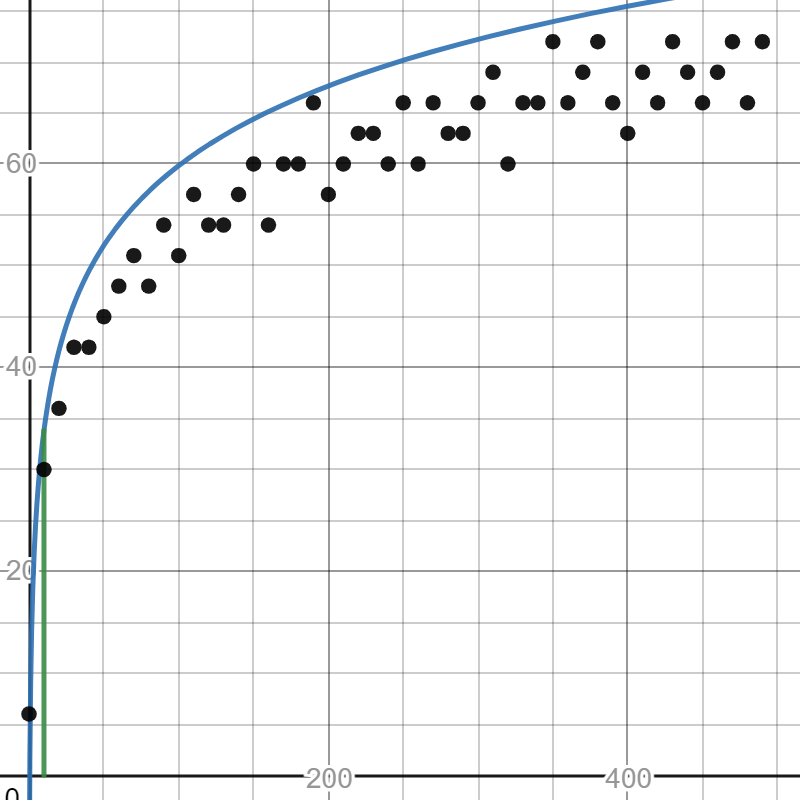
\includegraphics[width=10cm,height=5cm]{D2_P_WC.png}
        \end{picture}
    \end{figure}
    \vspace{-0.7cm}
    \begin{center}
        Figura 8. Gráfica de la función $f(n)=26\log_2(n)$.
    \end{center}
    \medskip
Podemos observar que algunos de estos puntos pasan por la función, y los demás están por debajo. De la definición de $O$:
\\ Necesitamos encontrar un $c_1g(n) \geq 26\log_2(n) $  $\forall n \geq n_1$, de ah\'i que:
\\ $26\log_2(n) \le 27\log_2(n) $ $\forall n \geq 10$, entonces $c_1 = 27$, $g(n)=\log_2(n)$, y $n_1=10$ $\therefore$ $f(n)=\log_2(n) \in O(\log_2(n))$.
\newpage
Para División3:
\\ Veamos en ejecución este algoritmo.
\begin{figure}[h]
    \vspace{3cm} \hspace{-2cm} \setlength{\unitlength}{1mm}
        \begin{picture}(15,25)(-35,0)
            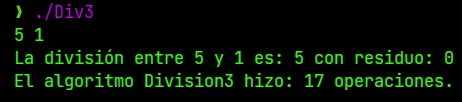
\includegraphics[width=10cm,height=5cm]{D3_Ex.jpg}
        \end{picture}
    \end{figure}
    \vspace{-0.7cm}
    \begin{center}
        Figura 9. Ejecución de Division3
    \end{center}
    \medskip
Ahora veamos su complejidad temporal a $priori$.
\begin{figure}[h]
    \vspace{3cm} \hspace{-2cm} \setlength{\unitlength}{1mm}
        \begin{picture}(15,25)(-35,0)
            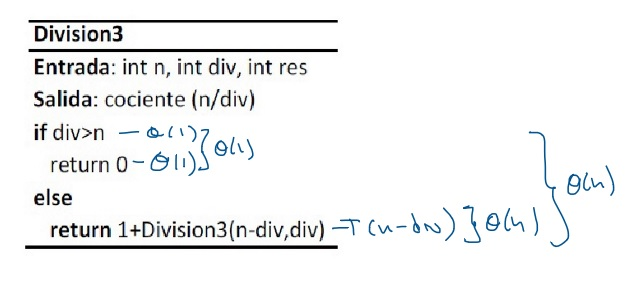
\includegraphics[width=10cm,height=5cm]{D3_PR.jpg}
        \end{picture}
    \end{figure}
    \vspace{-0.7cm}
    \begin{center}
        Figura 10. Análisis a $priori$ de Division3
    \end{center}
    \medskip
Ya que el peor caso es cuando $div$ vale 1, entonces la recurrencia es del tipo Decremento por 1, por lo tanto es lineal.
\newline
\\ Ahora realizaremos el análisis a $posteriori$
\\ Para el mejor caso:
\newpage
\begin{table}[htbp]
    \begin{center}
        \begin{tabular}{|c|c|}
            \hline
            \textbf{div} & \textbf{\# operaciones} \\
            \hline \hline
            0 &	2 \\ \hline
            10 & 2 \\ \hline
            20 &	2 \\ \hline
            30 &	2 \\ \hline
            40 &	2 \\ \hline
            50 &	2 \\ \hline
            60 & 2 \\ \hline
            70 & 2 \\ \hline
            80 & 2 \\ \hline
            90 & 2 \\ \hline
            100 & 2 \\ \hline
        \end{tabular}
        \caption{Mediciones para el mejor caso de Division3}
        \label{tabla:analisisDiv3BC}
    \end{center}
\end{table}
Así proponemos la función $f(n)=2$.
\begin{figure}[h]
    \vspace{3cm} \hspace{-2cm} \setlength{\unitlength}{1mm}
        \begin{picture}(15,25)(-35,0)
            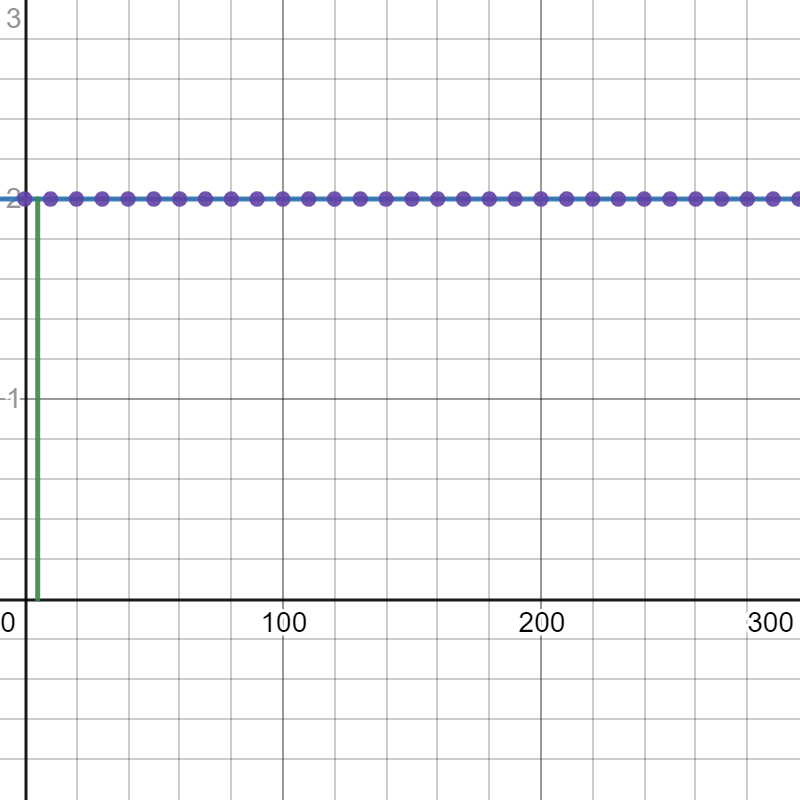
\includegraphics[width=10cm,height=5cm]{D3_P_BC.png}
        \end{picture}
    \end{figure}
    \vspace{-0.7cm}
    \begin{center}
        Figura 11. Gráfica de la función $f(n)=2$.
    \end{center}
    \medskip
Vemos que la función pasa por todos los puntos. De la definición de $\Omega$:
\\ Necesitamos encontrar un $c_1g(n) \le 2$  $\forall n \geq n_1$, de ah\'i que:
\\ $1(1) \le 2 $ $\forall n \geq 1$, entonces $c_1 = 1$, $g(n)=1$, y $n_1=1$ $\therefore$ $f(n)=2 \in \Omega(1)$.
\newpage
Para el peor caso:
\begin{table}[htbp]
    \begin{center}
        \begin{tabular}{|c|c|}
            \hline
            \textbf{div} & \textbf{\# operaciones} \\
            \hline \hline
            0 &	2 \\ \hline
            10 & 17 \\ \hline
            20 &	32 \\ \hline
            30 &	47 \\ \hline
            40 &	62 \\ \hline
            50 &	77 \\ \hline
            60 & 92 \\ \hline
            70 & 107 \\ \hline
            80 & 122 \\ \hline
            90 & 137 \\ \hline
            100 & 152 \\ \hline
        \end{tabular}
        \caption{Mediciones para el peor caso de Division3}
        \label{tabla:analisisDiv3WC}
    \end{center}
\end{table}
\\Así proponemos la función $f(n)= 2n$.
\begin{figure}[h]
    \vspace{3cm} \hspace{-2cm} \setlength{\unitlength}{1mm}
        \begin{picture}(15,25)(-35,0)
            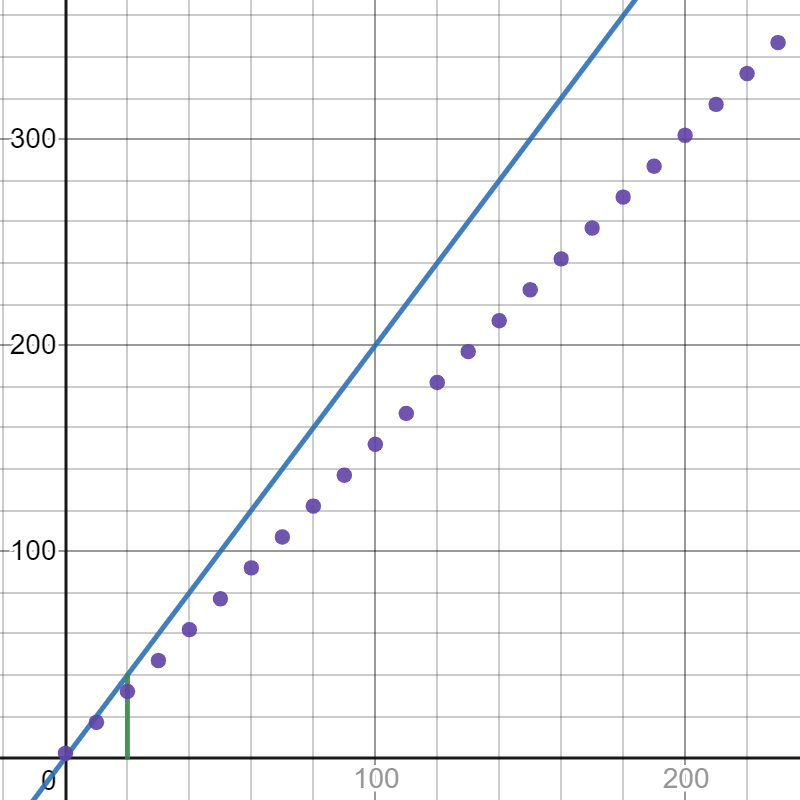
\includegraphics[width=10cm,height=5cm]{D3_P_WC.png}
        \end{picture}
    \end{figure}
    \vspace{-0.7cm}
    \begin{center}
        Figura 12. Gráfica de la función $f(n)=2n$.
    \end{center}
    \medskip
Podemos observar que algunos de estos puntos pasan por la función, y los demás están por debajo. De la definición de $O$:
\\ Necesitamos encontrar un $c_1g(n) \geq 2n $  $\forall n \geq n_1$, de ah\'i que:
\\ $2n \le 3n $ $\forall n \geq 20$, entonces $c_1 = 3$, $g(n)=n$, y $n_1=20$ $\therefore$ $f(n)=2n \in O(n)$.
\newline
\\ Vemos que el algoritmo recursivo Division3, es mejor que el algoritmo iterativo Division1, aunque por poco, sin embargo, el algoritmo iterativo Division2, es el mejor de los 3.
\newpage
Ahora veremos el segundo problema, de buscar un número en un arreglo de enteros. El tamaño del problema es el tamaño del arreglo, el mejor caso es cuando el valor que buscamos está en la posición del 1er tercio o en la posición del 2ndo tercio del arreglo, y el peor caso es cuando no está el valor en el arreglo.
\\ Así ahora veremos este problema en su versión recursiva.
\\ Veamos en ejecución este algoritmo.
\begin{figure}[h]
    \vspace{3cm} \hspace{-2cm} \setlength{\unitlength}{1mm}
        \begin{picture}(15,25)(-35,0)
            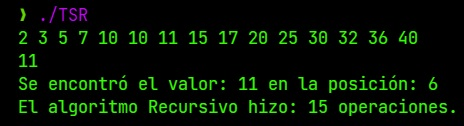
\includegraphics[width=10cm,height=5cm]{TSR_Ex.jpg}
        \end{picture}
    \end{figure}
    \vspace{-0.7cm}
    \begin{center}
        Figura 13. Ejecución de BusquedaEn3BloquesRecursiva
    \end{center}
    \medskip
Ahora veamos su complejidad temporal a $priori$.
\begin{figure}[h]
    \vspace{3cm} \hspace{-2cm} \setlength{\unitlength}{1mm}
        \begin{picture}(15,25)(-35,0)
            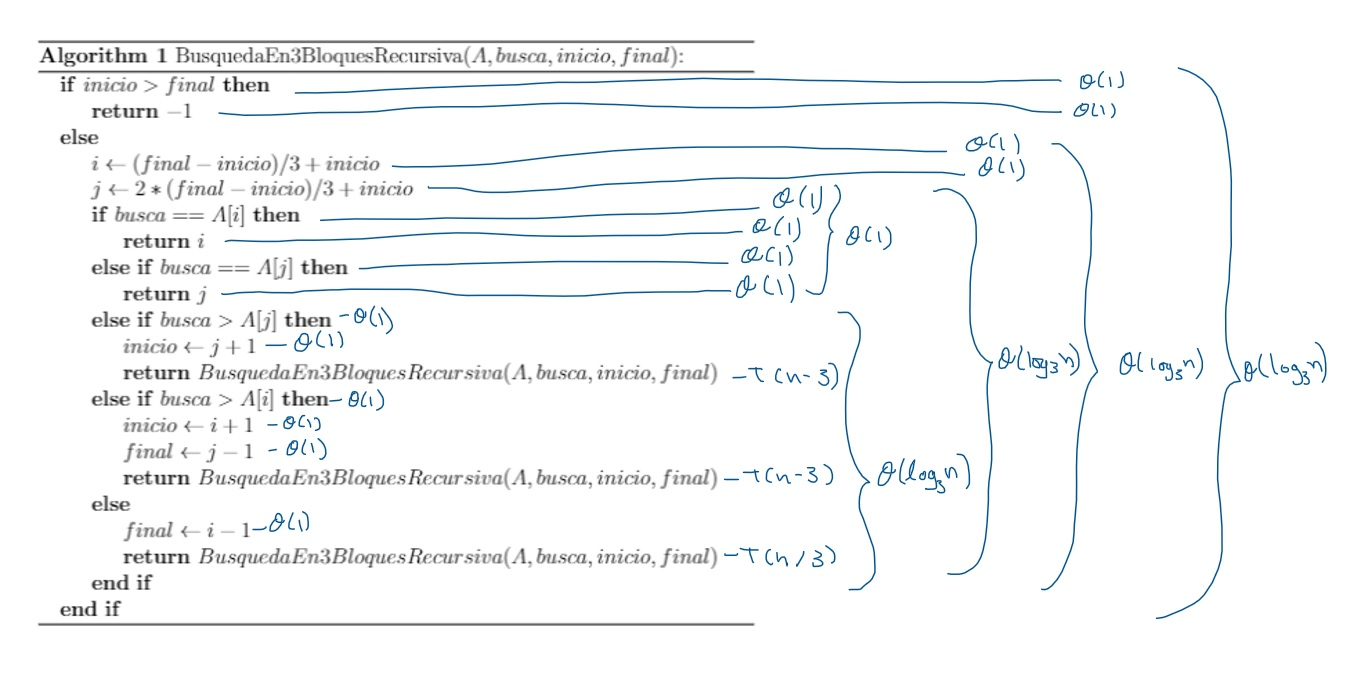
\includegraphics[width=10cm,height=5cm]{TSR_PR.jpg}
        \end{picture}
    \end{figure}
    \vspace{-0.7cm}
    \begin{center}
        Figura 14. Análisis a $priori$ de BusquedaEn3BloquesRecursiva
    \end{center}
    \medskip
Esta es una recursión del tipo Decremento por un factor constante, por lo tanto su complejidad es $\log_3n$.
\\ Ahora realizaremos el análisis a $posteriori$
\\ Para el mejor caso:
\newpage
\begin{table}[htbp]
    \begin{center}
        \begin{tabular}{|c|c|}
            \hline
            \textbf{n} & \textbf{\# operaciones} \\
            \hline \hline
            1 &	5 \\ \hline
            11 & 5 \\ \hline
            21 &	5 \\ \hline
            31 &	5 \\ \hline
            41 &	5 \\ \hline
            51 &	5 \\ \hline
            61 & 5 \\ \hline
            71 & 5 \\ \hline
            81 & 5 \\ \hline
            91 & 5 \\ \hline
            101 & 5 \\ \hline
        \end{tabular}
        \caption{Mediciones para el mejor caso de BusquedaEn3BloquesRecursiva}
        \label{tabla:analisisTSRBC}
    \end{center}
\end{table}
Así proponemos la función $f(n)=5$.
\begin{figure}[h]
    \vspace{3cm} \hspace{-2cm} \setlength{\unitlength}{1mm}
        \begin{picture}(15,25)(-35,0)
            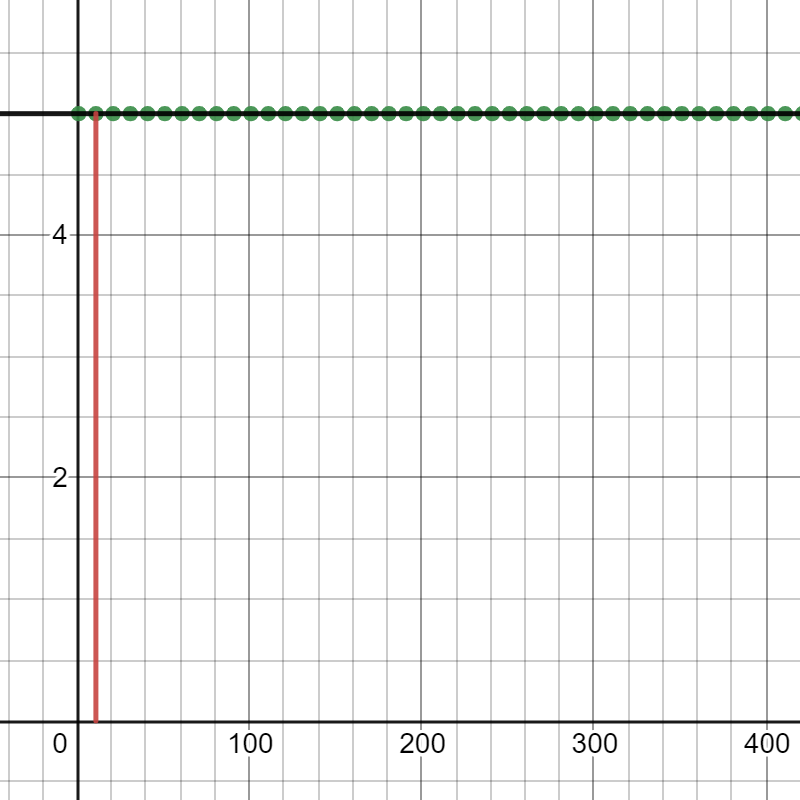
\includegraphics[width=10cm,height=5cm]{TSR_P_BC.png}
        \end{picture}
    \end{figure}
    \vspace{-0.7cm}
    \begin{center}
        Figura 15. Gráfica de la función $f(n)=5$.
    \end{center}
    \medskip
Vemos que la función pasa por todos los puntos. De la definición de $\Omega$:
\\ Necesitamos encontrar un $c_1g(n) \le 5$  $\forall n \geq n_1$, de ah\'i que:
\\ $4(1) \le 5 $ $\forall n \geq 1$, entonces $c_1 = 4$, $g(n)=1$, y $n_1=1$ $\therefore$ $f(n)=5 \in \Omega(1)$.
\newpage
Para el peor caso:
\begin{table}[htbp]
    \begin{center}
        \begin{tabular}{|c|c|}
            \hline
            \textbf{n} & \textbf{\# operaciones} \\
            \hline \hline
            1 &	11 \\ \hline
            11 & 28 \\ \hline
            21 &	29 \\ \hline
            31 &	28 \\ \hline
            41 &	42 \\ \hline
            51 &	29 \\ \hline
            61 & 38 \\ \hline
            71 & 39 \\ \hline
            81 & 45 \\ \hline
            91 & 42 \\ \hline
            101 & 38 \\ \hline
        \end{tabular}
        \caption{Mediciones para el peor caso de BusquedaEn3BloquesRecursiva}
        \label{tabla:analisisTSRWC}
    \end{center}
\end{table}
\\Así proponemos la función $f(n)= 20\log_3(n)$.
\begin{figure}[h]
    \vspace{3cm} \hspace{-2cm} \setlength{\unitlength}{1mm}
        \begin{picture}(15,25)(-35,0)
            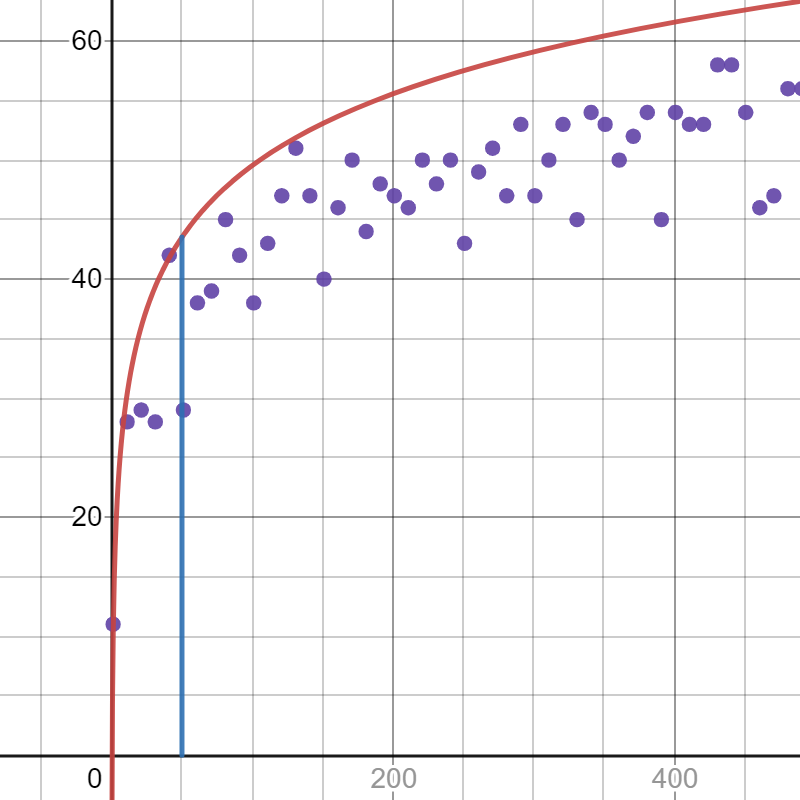
\includegraphics[width=10cm,height=5cm]{TSR_P_WC.png}
        \end{picture}
    \end{figure}
    \vspace{-0.7cm}
    \begin{center}
        Figura 16. Gráfica de la función $f(n)=20\log_3(n)$.
    \end{center}
    \medskip
Podemos observar que algunos de estos puntos pasan por la función, y los demás están por debajo. De la definición de $O$:
\\ Necesitamos encontrar un $c_1g(n) \geq 20\log_3(n) $  $\forall n \geq n_1$, de ah\'i que:
\\ $20\log_3(n) \le 21\log_3(n) $ $\forall n \geq 50$, entonces $c_1 = 21$, $g(n)=\log_3(n)$, y $n_1=50$ $\therefore$ $f(n)=20\log_3(n) \in O(\log_3(n))$.
\newpage
Ahora vamos a ver su versión iterativa.
\\ Veamos en ejecución este algoritmo.
\begin{figure}[h]
    \vspace{3cm} \hspace{-2cm} \setlength{\unitlength}{1mm}
        \begin{picture}(15,25)(-35,0)
            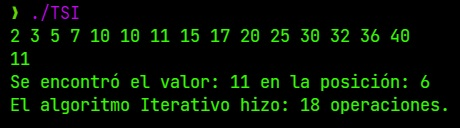
\includegraphics[width=10cm,height=5cm]{TSI_Ex.jpg}
        \end{picture}
    \end{figure}
    \vspace{-0.7cm}
    \begin{center}
        Figura 17. Ejecución de BusquedaEn3BloquesIterativa
    \end{center}
    \medskip
Ahora veamos su complejidad temporal a $priori$.
\begin{figure}[h]
    \vspace{3cm} \hspace{-2cm} \setlength{\unitlength}{1mm}
        \begin{picture}(15,25)(-35,0)
            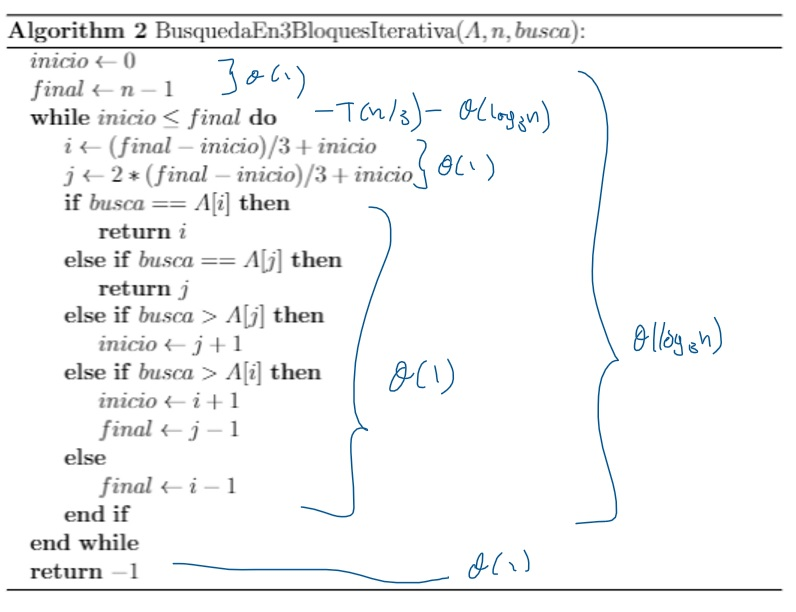
\includegraphics[width=10cm,height=5cm]{TSI_PR.jpg}
        \end{picture}
    \end{figure}
    \vspace{-0.7cm}
    \begin{center}
        Figura 18. Análisis a $priori$ de BusquedaEn3BloquesIterativa
    \end{center}
    \medskip
Este algoritmo genera la misma recurrencia, cabe recordar que las recurrencias no son propias de los algoritmos recursivos. Entonces al ser la misma que la del caso recursivo, será la misma complejidad también.
\\ Ahora realizaremos el análisis a $posteriori$
\\ Para el mejor caso:
\newpage
\begin{table}[htbp]
    \begin{center}
        \begin{tabular}{|c|c|}
            \hline
            \textbf{n} & \textbf{\# operaciones} \\
            \hline \hline
            1 &	9 \\ \hline
            11 & 9 \\ \hline
            21 &	9 \\ \hline
            31 &	9 \\ \hline
            41 &	9 \\ \hline
            51 &	9 \\ \hline
            61 & 9 \\ \hline
            71 & 9 \\ \hline
            81 & 9 \\ \hline
            91 & 9 \\ \hline
            101 & 9 \\ \hline
        \end{tabular}
        \caption{Mediciones para el mejor caso de BusquedaEn3BloquesIterativa}
        \label{tabla:analisisTSIBC}
    \end{center}
\end{table}
Así proponemos la función $f(n)=9$.
\begin{figure}[h]
    \vspace{3cm} \hspace{-2cm} \setlength{\unitlength}{1mm}
        \begin{picture}(15,25)(-35,0)
            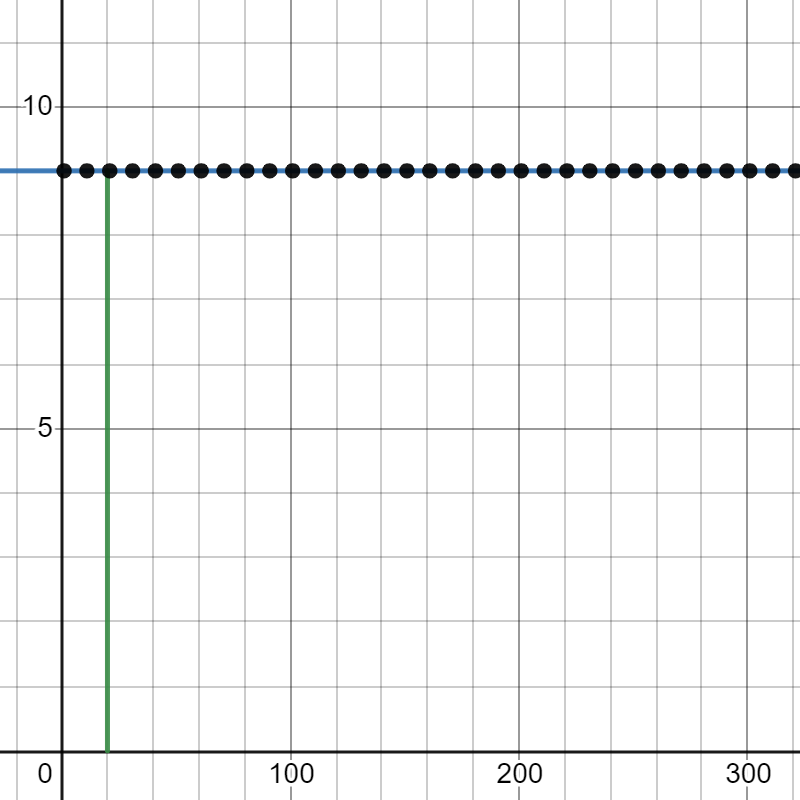
\includegraphics[width=10cm,height=5cm]{TSI_P_BC.png}
        \end{picture}
    \end{figure}
    \vspace{-0.7cm}
    \begin{center}
        Figura 19. Gráfica de la función $f(n)=9$.
    \end{center}
    \medskip
Vemos que la función pasa por todos los puntos. De la definición de $\Omega$:
\\ Necesitamos encontrar un $c_1g(n) \le 9$  $\forall n \geq n_1$, de ah\'i que:
\\ $8(1) \le 9 $ $\forall n \geq 1$, entonces $c_1 = 8$, $g(n)=1$, y $n_1=1$ $\therefore$ $f(n)=9 \in \Omega(1)$.
\newpage
Para el peor caso:
\begin{table}[htbp]
    \begin{center}
        \begin{tabular}{|c|c|}
            \hline
            \textbf{n} & \textbf{\# operaciones} \\
            \hline \hline
            1 &	13 \\ \hline
            11 & 27 \\ \hline
            21 &	34 \\ \hline
            31 &	34 \\ \hline
            41 &	41 \\ \hline
            51 &	41 \\ \hline
            61 & 41 \\ \hline
            71 & 41 \\ \hline
            81 & 41 \\ \hline
            91 & 41 \\ \hline
            101 & 41 \\ \hline
        \end{tabular}
        \caption{Mediciones para el peor caso de BusquedaEn3BloquesIterativa}
        \label{tabla:analisisTSIWC}
    \end{center}
\end{table}
\\Así proponemos la función $f(n)= 19\log_3(n)$.
\begin{figure}[h]
    \vspace{3cm} \hspace{-2cm} \setlength{\unitlength}{1mm}
        \begin{picture}(15,25)(-35,0)
            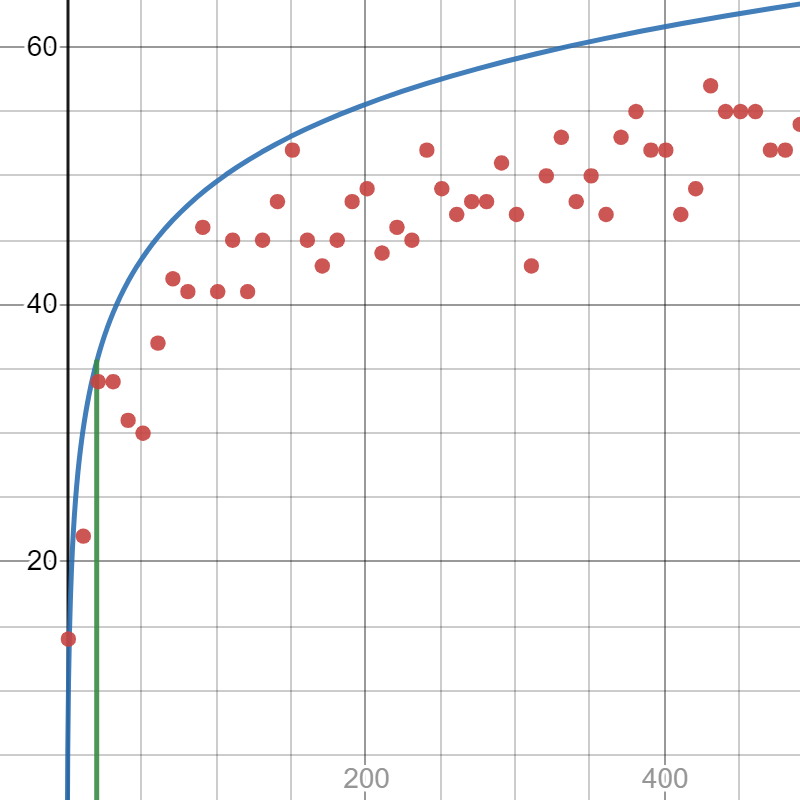
\includegraphics[width=10cm,height=5cm]{TSI_P_WC.png}
        \end{picture}
    \end{figure}
    \vspace{-0.7cm}
    \begin{center}
        Figura 20. Gráfica de la función $f(n)=19\log_3(n)$.
    \end{center}
    \medskip
Podemos observar que algunos de estos puntos pasan por la función, y los demás están por debajo. De la definición de $O$:
\\ Necesitamos encontrar un $c_1g(n) \geq 19\log_3(n) $  $\forall n \geq n_1$, de ah\'i que:
\\ $19\log_3(n) \le 20\log_3(n) $ $\forall n \geq 50$, entonces $c_1 = 20$, $g(n)=\log_3(n)$, y $n_1=50$ $\therefore$ $f(n)=19\log_3(n) \in O(\log_3(n))$.
\newline
\\ Vemos que ambos algoritmos tienen la misma complejidad, sin embargo el recursivo hace menos operaciones para el mejor caso, pero el iterativo parece mejor cuando el peor caso, así que para decir cuál sería mejor, se podría decir que el iterativo, puesto que no ocupa espacio extra, y es mejor para el peor caso, que es probable que se presente más veces que el mejor caso.


\newpage
\section{Conclusiones}
\textbf{Conclusi\'on General}
\\ Para encontrar las complejidades de algunos ciclos de los algoritmos fue complicado observar cuál era la complejidad, hasta que se encontró cuál era el peor caso y mejor caso, y tratarlos de manera separada. Los algoritmos funcionan bien, así que podemos decir que los resultados fueron los esperados, todos tienen complejidades aceptables, aunque quizás el algoritmo de búsqueda en 3 bloques podría ser mejor si fuera $\log_2n$ puesto que crece menos rápido que $\log_3n$.
\\
\\
\textbf{Conclusi\'on de Anthony}

\begin{wrapfigure}{r}{5.5cm}
    
\includegraphics[width=5.5cm]{me.jpg}
\end{wrapfigure} 
Esta práctica en lo personal me gustó bastante, los temas fueron realmente interesantes, creo que resolver recurrencias puede llegar a ser divertido, es un tema muy interesante, en especial las recurrencias no homogéneas, puesto que se pueden encontrar recurrencias, y resolverlas, que probablemente no puedan ser vistas en algún algoritmo, y regresa esta abstracción tan interesante que se encuentra regularmente en las matemáticas, de resolver cosas tan abstractas que no puedan ser vistas en práctica, o que no puedan ni imaginarse. Y aunque generalmente los algoritmos recursivos ocupan mucha memoria, me llama mucho la atención lo elegante que se puede llegar a escribir un problema, cuando se representa de forma recursiva; y el hecho de existan muchas funciones recursivas de distintas categorías que pueden resolver el problema, me da mucha curiosidad.
\newpage
\section{Anexo}
Para este caso no se realizaron problemas de tarea para anexar.

\section{Bibliograf\'ia}
Dillig, I. CS 311H. Revisado Marzo 27, 2022, de $https://www.cs.utexas.edu/~isil/cs311h/$
\newline
Rubio-Sanchez, M, (2018). Introduction to Recursive Programming. CRC Press.
\medskip

\end{document}